\definecolor{gold}{rgb}{0.77,0.69,0.37}
\newlength{\hptitlewidth}
\newlength{\rationalh}
\newcommand{\hptitle}[2][\stockwidth]{%
  \setlength{\hptitlewidth}{#1}%
  \centering\color{white}%
  \vskip 3cm\resizebox{.95\hptitlewidth}{!}{\textls[100]{HARRY POTTER AND THE}}%
  \vskip 2mm%
  \color{gold}%
  \settoheight{\rationalh}{\resizebox{.95\hptitlewidth}{!}{\textls[20]{RATIONALITY}}}
  \resizebox{!}{0.9\rationalh}{\textls[50]{METHODS}}%
  \hfil\resizebox{!}{0.3\rationalh}{\textls[50]{Of}}%
  \vskip 2mm%
  \resizebox{.95\hptitlewidth}{!}{\textls[20]{RATIONALITY}}%
  \vskip 8mm%
  \color{white}%
  \resizebox{.5\hptitlewidth}{!}{\textls[50]{\scshape{}Fanfiction by Eliezer Yudkowsky}}%
  \vfill%
  \textls[50]{\scshape #2}%
  \color{black}%
  \vskip 1cm\ %
}
\providecommand{\fullvolumetitle}[1]{Book #1: \volumetitle}

\ifcover%
\definecolor{backgroundcover}{HTML}{272c36}
\newpagecolor{backgroundcover}\afterpage{\restorepagecolor}
\newcommand\BackgroundPic{
\put(0,0){%
\parbox[b][\paperheight]{\paperwidth}{%
\vfill%
\centering%
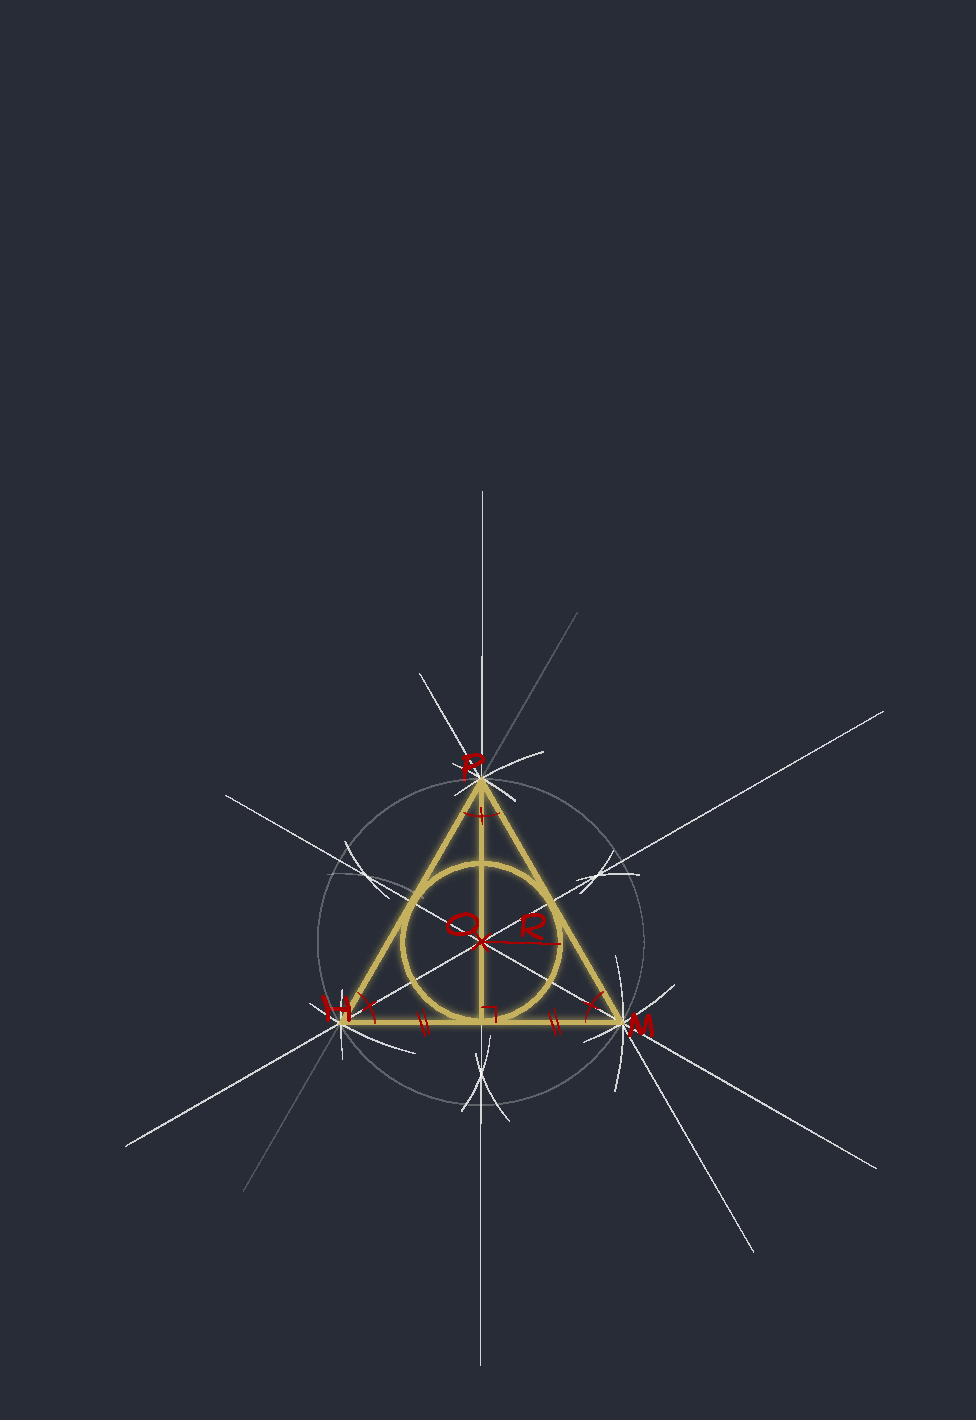
\includegraphics[width=\paperwidth,height=\paperheight,keepaspectratio]{cover1.pdf}%
\vfill%
}}}\AddToShipoutPicture*{\BackgroundPic}%
\AddToShipoutPicture*{\put(0,0){%
\parbox[b][\paperheight]{\paperwidth}{%
\hptitle{\fullvolumetitle{\volumenumber}}%
}}}%
\ %
\cleartorecto
\fi
\begin{center}
\thispagestyle{empty}
{\hpfont
\Huge\MakeUppercase{Harry Potter}\vspace*{0.5cm}

\Large\MakeUppercase{et les Méthodes de la Rationalité} %

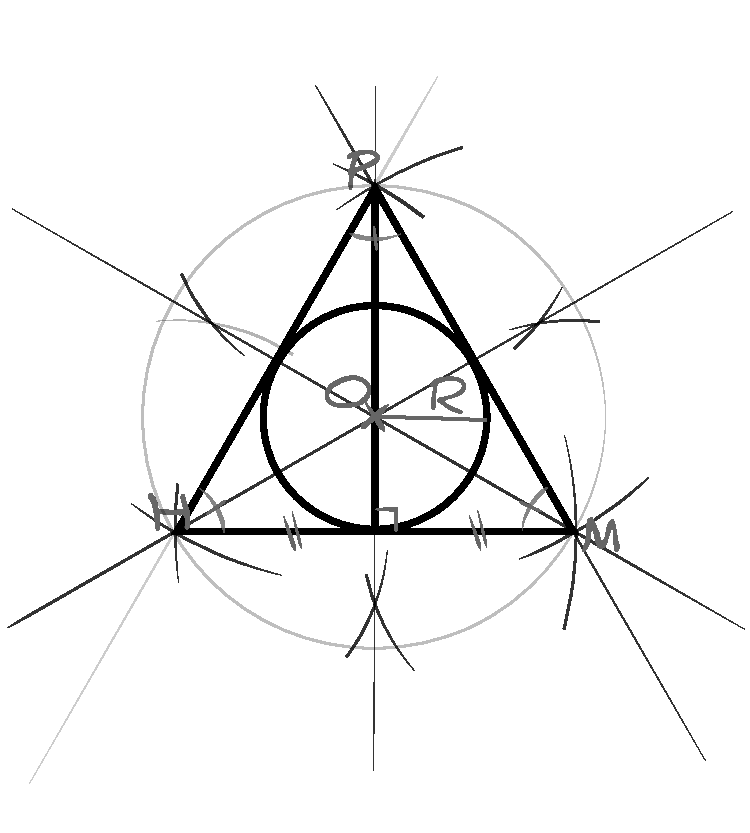
\includegraphics[scale=0.5]{bubble.pdf}

\Large Fanfiction par \vspace*{.25cm}

\huge \MakeUppercase{Eliezer Yudkowsky}%

\normalsize

\vspace*{1\baselineskip}
\fullvolumetitle{\volumenumber}
}

\vspace{1cm}
Retrouvez le livre en ligne, avec les notes de l'auteur, fanarts et autres informations sur : \url{http://hpmor.com} \\

\vspace{1cm}
Traduction~: AdrianH\\
-\\
Adaptation et corrections~: Anthony CARRÉ\\
\url{https://github.com/yekcim/hpmor}


\end{center}

\cleartoverso

\begin{center}
\vspace*{2cm}

\thispagestyle{empty}
Basé sur les personnages de

\vspace*{.5cm}

\Large \MakeUppercase{J. K. Rowling} \normalsize

\vspace*{.5cm}

et ses livres:

\vspace*{.5cm}

{
        \newcounter{books_list_counter}
        \def \hpBook #1{
                \addtocounter{books_list_counter}{1}
                \textit{Harry Potter #1} \par
                Année \numtoName{\value{books_list_counter}} à Poudelard
                \smallskip\par
        }
        \hpBook{à l'école des sorciers}
        \hpBook{et la Chambre des secrets}
        \hpBook{et le Prisonnier d'Azkaban}
        \hpBook{et la Coupe de feu}
        \hpBook{et l'Ordre du Phénix}
        \hpBook{et le Prince de sang-mêlé}
        \hpBook{et les Reliques de la Mort}
}
\end{center}
\cleartorecto% FIXME: For some reason, without this the contents ends up on a verso page (an extra blank page is added)



